\documentclass[10pt, a4paper]{article}
\usepackage{cmap}
\usepackage[T2A]{fontenc}
\usepackage[utf8]{inputenc}
\usepackage[english, russian]{babel}
\usepackage[dvipsnames,table,xcdraw]{xcolor}
\usepackage{
	amsmath,
	amssymb,
	scrextend,
	enumitem,
	pscyr,
	multicol,
	cmap,
	titling,
	indentfirst,
	cancel,
	wrapfig,
	gensymb,
	tikz,
	graphicx,
	fancyhdr,
	mathrsfs,
	graphbox,
	indentfirst
}
%Параметры страницы
\usepackage[left=15mm,right=15mm,
top=2cm,bottom=2cm]{geometry}
\pagestyle{fancy}
%Путь к картинкам
\graphicspath{{pic/}}
\DeclareGraphicsExtensions{.pdf,.png,.jpg}
%Числа в списке второго уровня по умолчанию
\renewcommand{\labelenumii}{\arabic{enumii})}
%Новые команды
\definecolor{silver}{rgb}{0.7, 0.7, 0.7}
\definecolor{dark}{rgb}{0.3, 0.3, 0.3}
\definecolor{harvestgold}{rgb}{0.85, 0.57, 0.0}
\newcommand{\answer}[1]{\textcolor{silver}{\fbox{#1}}}
\newcommand{\ranswer}[1]{\textcolor{silver}{\begin{flushright}\vspace{-1em}\fbox{#1}\end{flushright}}}
\newcommand{\leveli}{\textcolor{dark}{$\blacksquare\square\square$}\hspace{0.5em}}
\newcommand{\levelii}{\textcolor{dark}{$\blacksquare\blacksquare\square$}\hspace{0.5em}}
\newcommand{\leveliii}{\textcolor{dark}{$\blacksquare\blacksquare\blacksquare$}\hspace{0.5em}}

%Русские символы в списке
\AddEnumerateCounter{\asbuk}{\russian@alph}{щ}

%Сеттеры
\setlength{\parindent}{5ex}
\setlength{\parskip}{1em}

\begin{document}
		
\lhead{Функции}
\rhead{Школа <<Симметрия>>}

\section{Линейная функция}
\begin{enumerate}
	
	\item \leveli Найдите уравнение прямой, которая проходит через начало координат и точку $(4;2)$. \ranswer{$y=0,5x$}
	\item \leveli Найдите уравнение прямой, которая проходит через начало координат и точку $(-2;2)$. \ranswer{$y=-x$}
	\item \leveli Найдите уравнение прямой, которая проходит через начало координат и точку $(-5;1)$. \ranswer{$y=-0,2x$}
	\item \leveli Найдите уравнение прямой, которая проходит через начало координат и точку $(-4;-3)$. \ranswer{$y=0,75x$}
	\item \leveli Найдите уравнение прямой, которая проходит через начало координат и точку $(-1;-4)$. \ranswer{$y=4x$}
	\item \leveli Найдите уравнение прямой, которая проходит через точки с координатами $(4;6)$ и $(-8;-3)$. \ranswer{$y=0,75x+3$}
	\item \leveli Найдите уравнение прямой, которая проходит через точки с координатами $(6;4)$ и $(-6;1)$. \ranswer{$y=0,25x+2,5$}
	\item \leveli Найдите уравнение прямой, которая проходит через точки с координатами $(-2;-2)$ и $(0;4)$. \ranswer{$y=3x+4$}
	\item \leveli Найдите уравнение прямой, которая проходит через точки с координатами $(3;1)$ и $(-10;-3)$. \ranswer{$y=0,7x+0,5$}
	\item \leveli Принадлежит ли точка с координатами $(1;4)$ уравнению прямой $y=4x$? \ranswer{Да}
	\item \leveli Принадлежит ли точка с координатами $(3,5;2)$ уравнению прямой $y=\frac{2}{3}x$? \ranswer{Нет}
	\item \leveli Принадлежит ли точка с координатами $(7,5;2,5)$ уравнению прямой $y=\frac{1}{3}x$? \ranswer{Да}
	\item \leveli Принадлежит ли точка с координатами $(-5;-2)$ уравнению прямой $y=0,75x+3$? \ranswer{Нет}
	\item \leveli Принадлежит ли точка с координатами $(-3;-8)$ уравнению прямой $y=2x-2$? \ranswer{Да}
	\item \leveli Принадлежит ли точка с координатами $(-2;-4)$ уравнению прямой $y=2x-2$? \ranswer{Нет}
	\item \leveli Принадлежит ли точка с координатами $(2;1)$ уравнению прямой $y=3x-5$? \ranswer{Да}
	\item \leveli Принадлежит ли точка с координатами $(3;5)$ уравнению прямой $y=3x-5$? \ranswer{Нет}
	\item \leveli Выяснить, лежат ли точки $A(-2;-2)$, $B(10;4)$ и $C(17;10)$ на одной прямой. \ranswer{Нет}
	\item \leveli Выяснить, лежат ли точки $A(6;-6)$, $B(10;10)$ и $C(12;18)$ на одной прямой. \ranswer{Да}
	\item \leveli Выяснить, лежат ли точки $A(-11;6)$, $B(-6;3)$ и $C(4;-3)$ на одной прямой. \ranswer{Да}
	\item \leveli Выяснить, лежат ли точки $A(-11;6)$, $B(-6;3)$ и $C(9;-6)$ на одной прямой. \ranswer{Да}
	\item \leveli Выяснить, лежат ли точки $A(-11;6)$, $B(4;-5)$ и $C(-6;3)$ на одной прямой. \ranswer{Нет}
	\item \leveli Найдите координаты точки пересечения пересечения прямых $y=\dfrac{1}{2}x$ и $y=x+4$. \ranswer{$(-8;-4)$}
	\item \leveli Найдите координаты точки пересечения пересечения прямых $y=x$ и $y=1,5x+5$. \ranswer{$(-10;-10)$}
	\item \leveli Найдите координаты точки пересечения пересечения прямых $y=0,5x+3$ и $y=-\dfrac{1}{3}x$. \ranswer{$(-3,6;1,2)$}
	\item \leveli Найдите координаты точки пересечения пересечения прямых $y=x+4$ и $y=-2$. \ranswer{$(-6;-2)$}
	\item \leveli Найдите координаты точки пересечения пересечения прямых $y=-2x-8$ и $y=6$. \ranswer{$(-7;6)$}
	\item \leveli Найдите координаты точки пересечения пересечения прямых $y=-x-2$ и $y=4$. \ranswer{$(-6;4)$}
	\item \leveli Найдите координаты точки пересечения пересечения прямых $y=\dfrac{2}{3}x-4$ и $y=4$. \ranswer{$(12;4)$}
	\item \leveli Найдите координаты точки пересечения пересечения прямых $y=0,25x-4$ и $y=2$. \ranswer{$(24;2)$}
	\item \levelii Найдите координаты точки пересечения пересечения прямых $y=3x-5$ и $y=\dfrac{3}{5}x+7$. \ranswer{$(5;10)$}
	\item \levelii Найдите координаты точки пересечения пересечения прямых $y=3x-5$ и $y=-\dfrac{1}{3}x+5$. \ranswer{$(3;4)$}
	\item \levelii Найдите координаты точки пересечения пересечения прямых $y=x-2$ и $y=0,5x+6$. \ranswer{$(16;14)$}
	\item \levelii Найдите координаты точки пересечения пересечения прямых $y=-0,5x-2$ и $y=0,5x+8$. \ranswer{$(-10;3)$}
	\item \levelii Найдите координаты точки пересечения пересечения прямых $y=x+4$ и $y=-0,25x-3$. \ranswer{$(-5,6;-1,6)$}
	\item \levelii Выяснить, можно ли через точки $A(-6;6)$, $B(2;-8)$, $C(-8;-2)$ и $D(14;-6)$ провести две параллельные прямые. \ranswer{Да, можно}
	\item \levelii Выяснить, можно ли через точки $A(-8;0)$, $B(8;4)$, $C(0;-6)$ и $D(8;-4)$ провести две параллельные прямые. \ranswer{Да, можно}
	\item \levelii Выяснить, можно ли через точки $A(-6;-2)$, $B(8;6)$, $C(-8;-8)$ и $D(8;-4)$ провести две параллельные прямые. \ranswer{Нет, нельзя}
	\item \leveli Найдите уравнение прямой, которая проходит через точку $(-5;3)$ и параллельна прямой $y=-x+4$. \ranswer{$y=-x-2$}
	\item \leveli Найдите уравнение прямой, которая проходит через точку $(3;-1)$ и параллельна прямой $y=\dfrac{1}{5}x+4$. \ranswer{$y=\frac{1}{2}x-2,5$}
	\item \leveli Найдите уравнение прямой, которая проходит через точку $(5;-0,5)$ и параллельна прямой $y=-0,25x+3,5$. \ranswer{$y=-0,25x+0,75$}
	\item \leveli Найдите уравнение прямой, которая проходит через точку $(3;0)$ и параллельна прямой $y=-2x+3,5$. \ranswer{$y=-2x+6$}
	\item \leveli Найдите уравнение прямой, которая проходит через точку $(3;1,5)$ и параллельна прямой $y=-1\dfrac{2}{3}x+2,5$. \ranswer{$y=-1\frac{2}{3}x+6,5$}
	\item \levelii Найдите уравнение прямой, которая проходит через точку $(3;2)$ и перпендикулярна прямой $y=-2x+2$. \ranswer{$y=0,5x+0,5$}
	\item \levelii Найдите уравнение прямой, которая проходит через точку $(6;0)$ и перпендикулярна прямой $y=-0,5x-0,5$. \ranswer{$y=2x-12$}
	\item \levelii Найдите уравнение прямой, которая проходит через точку $(0,5;-1,5)$ и перпендикулярна прямой $y=-\dfrac{2}{3}x+2$. \ranswer{$y=1,5x-2,25$}
	\item \levelii Найдите уравнение прямой, которая проходит через точку $(4,5;-0,5)$ и перпендикулярна прямой $y=-\dfrac{3}{4}x-\dfrac{1}{2}$. \ranswer{$y=\frac{4}{3}x-6,5$}
	\item \levelii Найдите координаты точки пересечения двух перпендикулярных прямых, если известно, что первая прямая задана уравнением $y=-0.25x-1.5$, а вторая проходит через точку $(6,5;1)$. \ranswer{$(6;-3)$}
	\item \levelii Найдите координаты точки пересечения двух перпендикулярных прямых, если известно, что первая прямая задана уравнением $y=-\dfrac{2}{3}x-1.5$, а вторая проходит через точку $(6;1)$. \ranswer{$(3;-3,5)$}
	\item \levelii Найдите координаты точки пересечения двух перпендикулярных прямых, если известно, что первая прямая задана уравнением $y=-3x+1$, а вторая проходит через точку $(6;-2)$. \ranswer{$(1,5;-3,5)$}
	\item \leveliii Известно, что точки $A(10;-4)$, $B(4;2)$ и $C(8;6)$, а $ABCD$ --- прямоугольник. Найдите координаты точки $D$. \ranswer{$(14;0)$}
	\item
	\begin{minipage}[t]{0.6\textwidth}
		\leveli Прямые $f(x)=x-5,5$ и $g(x)$ пересекаются в точке с координатами $(a;b)$. Найдите $a+b$. \ranswer{$-10$}
	\end{minipage}
	\begin{minipage}[t]{0.3\textwidth}
		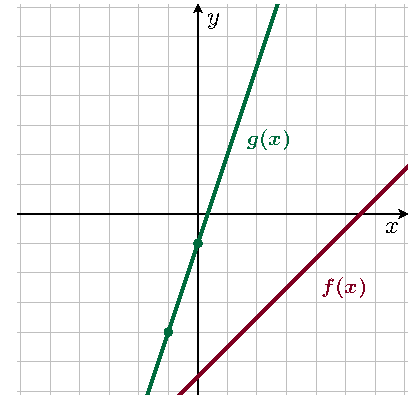
\includegraphics[align=t, width=\textwidth]{../graphs/graph_6/graph_6}
	\end{minipage}
	\item
	\begin{minipage}[t]{0.6\textwidth}
		Найдите координаты точки пересечения прямых $f(x)$ и $g(x)$. В ответ запишите сумму абсциссы и ординаты. \ranswer{$3,75$}
	\end{minipage}
	\begin{minipage}[t]{0.3\textwidth}
		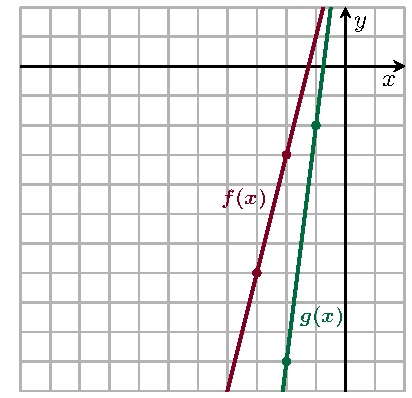
\includegraphics[align=t, width=\textwidth]{../graphs/graph_5/graph_5}
	\end{minipage}
\end{enumerate}
\section{Параболы}
\begin{enumerate}
	\item
	\begin{minipage}[t][8cm][t]{0.5\textwidth}
		На рисунке изображен график функции вида $y=ax^2+bx+c$, где числа $a$, $b$ и $c$ — целые. Вычислите $f\left(\dfrac{1}{4}\right)-f\left(\dfrac{1}{2}\right)$.
		\begin{flushright}
			\rotatebox{180}{\fbox{$-0,3125$}}
		\end{flushright}
	\end{minipage}
	\begin{minipage}[t][8cm][t]{0.5\textwidth}
		\hspace{10pt}
		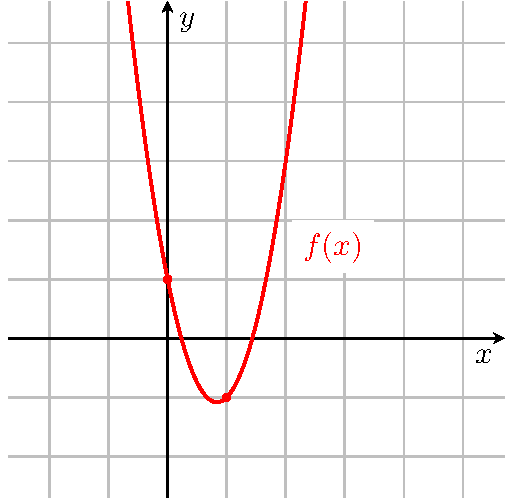
\includegraphics[align=t, width=0.8\textwidth]{graphs/graph_1/graph_1}
	\end{minipage}
\end{enumerate}
\section{Гиперболы}
\begin{enumerate}
	\item 
	\begin{minipage}[t][8cm][t]{0.5\textwidth}
		На рисунке изображен график функции вида $y=\dfrac{a}{x+b}+c$, где числа $a$, $b$ и $c$ — целые. Найдите $f\left(-\dfrac{8}{5}\right)$.
		\begin{flushright}
			\rotatebox{180}{\fbox{$-1\dfrac{1}{3}$}}
		\end{flushright}
	\end{minipage}
	\begin{minipage}[t][8cm][t]{0.5\textwidth}
		\hspace{10pt}
		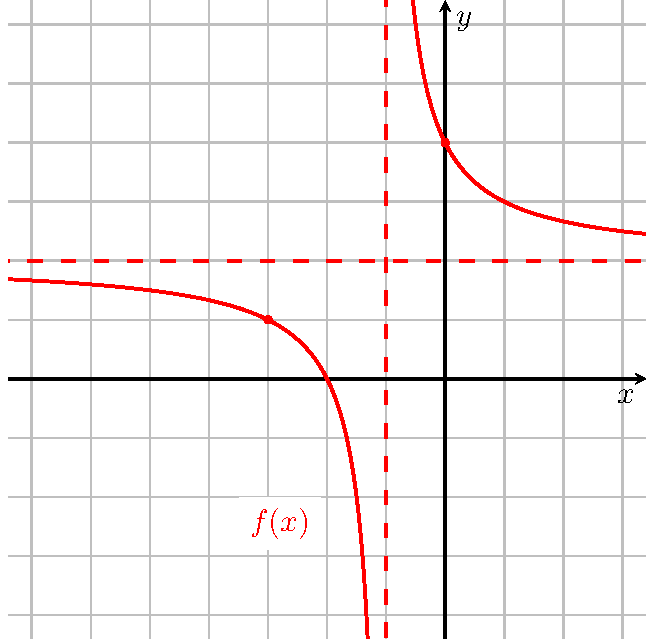
\includegraphics[align=t, width=0.8\textwidth]{graphs/graph_2/graph_2}
	\end{minipage}
	
\end{enumerate}
\end{document}